\documentclass{tufte-handout}

\title{Od: Lorenz-system-based voltages for the Music Thing Modular Workshop System Computer
\thanks{musicthing.co.uk/workshopsystem}}

\author[mcclintic.sphere.fx]{mcclintic.sphere.fx}

%\date{28 March 2010} % without \date command, current date is supplied

%\geometry{showframe} % display margins for debugging page layout

\usepackage{graphicx} % allow embedded images
  \setkeys{Gin}{width=\linewidth,totalheight=\textheight,keepaspectratio}
  \graphicspath{{graphics/}} % set of paths to search for images
\usepackage{amsmath}  % extended mathematics
\usepackage{booktabs} % book-quality tables
\usepackage{units}    % non-stacked fractions and better unit spacing
\usepackage{multicol} % multiple column layout facilities
\usepackage{lipsum}   % filler text
\usepackage{fancyvrb} % extended verbatim environments
  \fvset{fontsize=\normalsize}% default font size for fancy-verbatim environments

% Standardize command font styles and environments
\newcommand{\doccmd}[1]{\texttt{\textbackslash#1}}% command name -- adds backslash automatically
\newcommand{\docopt}[1]{\ensuremath{\langle}\textrm{\textit{#1}}\ensuremath{\rangle}}% optional command argument
\newcommand{\docarg}[1]{\textrm{\textit{#1}}}% (required) command argument
\newcommand{\docenv}[1]{\textsf{#1}}% environment name
\newcommand{\docpkg}[1]{\texttt{#1}}% package name
\newcommand{\doccls}[1]{\texttt{#1}}% document class name
\newcommand{\docclsopt}[1]{\texttt{#1}}% document class option name
\newenvironment{docspec}{\begin{quote}\noindent}{\end{quote}}% command specification environment

\begin{document}

\maketitle% this prints the handout title, author, and date

\begin{abstract}
\noindent
Od is a program for the Music Thing Modular Workshop System Computer
module that simulates the Lorenz system in order to produce loop-able 
control voltage and pulse signals that display sensitivity to initial conditions.
\end{abstract}

%\printclassoptions

\section{The Lorenz System}\label{sec:the-lorenz-system}

\newthought{The Lorenz system\sidenote{Lorenz, E.N. (1963) \textit{Deterministic Nonperiodic Flow}. Journal of Atmospheric Sciences, 20, 130-141} is a set of} three coupled, first-order ordinary differential equations (ODEs).

$$\frac{dx}{dt} = \sigma(y - x)$$

$$\frac{dy}{dt} = x(\rho - z) - y$$

$$\frac{dz}{dt} = x y - \beta z$$

Here, $x$, $y$ and $z$ are the "coordinates" of the system, their evolution through a three-dimensional space as a function of time are the solutions to the set of differential equations, and will be referred to as "trajectories" herein.

\begin{figure*}[h]
  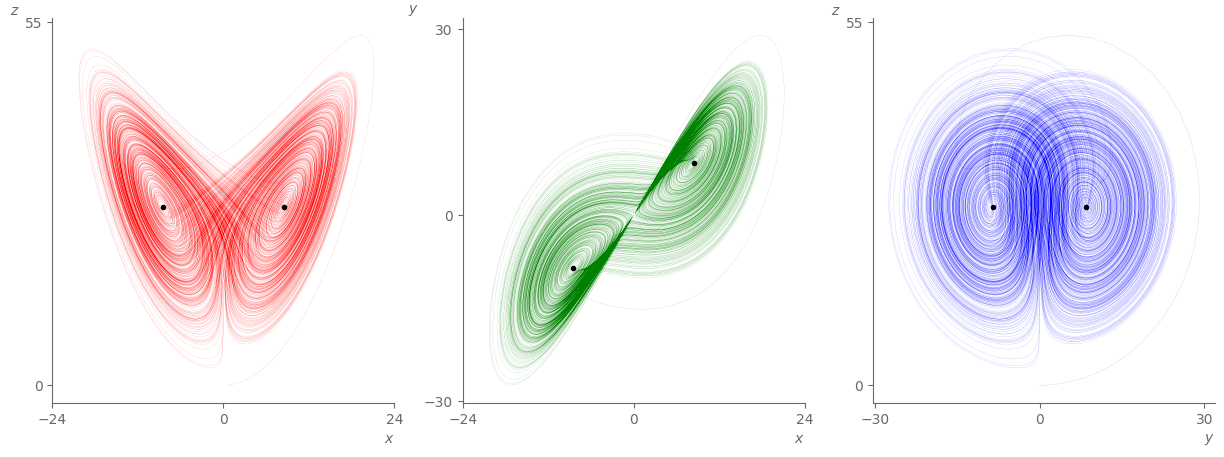
\includegraphics[width=\linewidth]{lorenz_attractor.png}%
  \caption{Trajectories of the Lorenz attractor projected onto each Cartesian plane. The two fixed point attractors are shown as gray dots.}%
  \label{fig:fullfig}%
\end{figure*}

Three constants $\rho$, $\beta$ and $\sigma$ determine the overall behaviour of the system. For values of $\rho < 1$, all trajectories converge to the origin ($x, y, z = 0$). At $\rho=1$, a bifurcation occurs such that for values of $\rho > 1$ there are a pair of fixed point attractors (see Fig. 1), and all trajectories will evolve towards one of the two. 

For the specific values $\sigma=10$, $\beta=8/3$, $\rho=28$ the system exhibits chaotic behaviour, and corresponds to the "Lorenz Attractor" (see Citation 2). Trajectories of this system will propagate forever, never repeating or converging.


\begin{figure*}[h]
  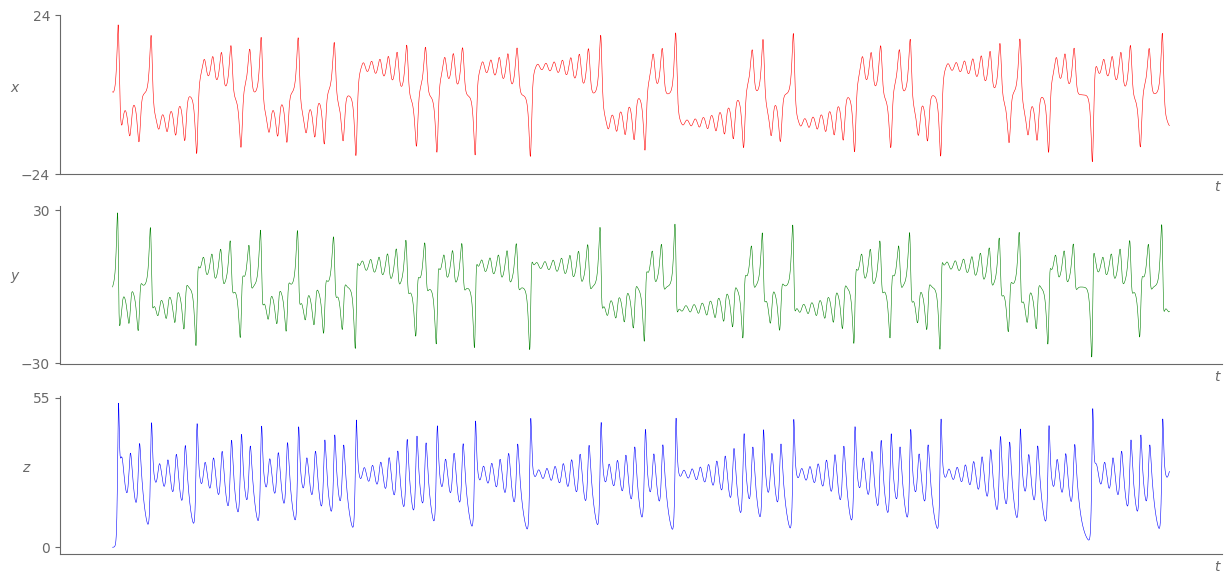
\includegraphics[width=\linewidth]{control_voltages.png}%
  \caption{The first 10,000 steps of trajectories of the Lorenz attractor along each Cartesian axis, as a function of time. Note the similarity of the $x$ and $y$ traces. The $x$ and $z$ traces correspond to the CV outputs of the module. Times at which the $x$-coordinate crosses zero are marked with black dots.}%
  \label{fig:control_voltages}%
\end{figure*}

In order to generate trajectories of the type shown in Fig. 2 to be used as control voltages (CVs), the system of differential equations must be solved.

\subsection{Solving the System}\label{sec:solving_the_system}

The solution of the system of ODEs is an "initial value problem" \sidenote[][0.5cm]{Press, W. H., Teukolsky, S. A., Vetterling, W. T. and Flannery, B. P. (2007) \textit{Numerical Recipes 3rd Edition: The Art of Scientific Computing}}. That is, the coordinates of an initial point are given, and the goal is (in general) to find the values $x$, $y$, $z$ at some discrete list of future time values. In this specific case, the goal is to be able to continually determine the next step in the trajectory so that the functions $x$, $y$ and $z$ can be exported as control voltage via the Computer's CV output sockets.
The simplest approach to solution of an initial value problem is the "Euler method"\sidenote{Euler, L. (1768) \textit{Institutiones calculi integralis}}, which discretizes time into individual constant steps, $\Delta t$, allowing the next point on a trajectory to be obtained via a simple formula.

$$x_{n+1} = x_n + \Delta t f_{x}(t, x, y, z)$$

The error introduced by this approach is on the order of ${\Delta t}^2$. For most scientific applications, this approach is woefully poor. However, when generating solutions for musical purposes, trajectories that have the appropriate character are sufficient, and so the simplest (and computationally cheapest) approach has been relied upon for Od.

\section{The Module}\label{sec:the_module}

\newthought{The module itself utilizes} a pair of Lorenz systems ($A$ and $B$) which run concurrently at different rates. Inspired by the \o chd module\sidenote{https://www.instruomodular.com/product/ochd/}, the relative rate is fixed at a musically engaging ratio (in this case, $\Delta t_{fast} = \frac{11}{5} \Delta t_{slow}$. The overall rate is controlled by the main knob or the left-most CV input, depending on whether a jack is plugged into the left-most CV input.

\begin{figure}[h]
  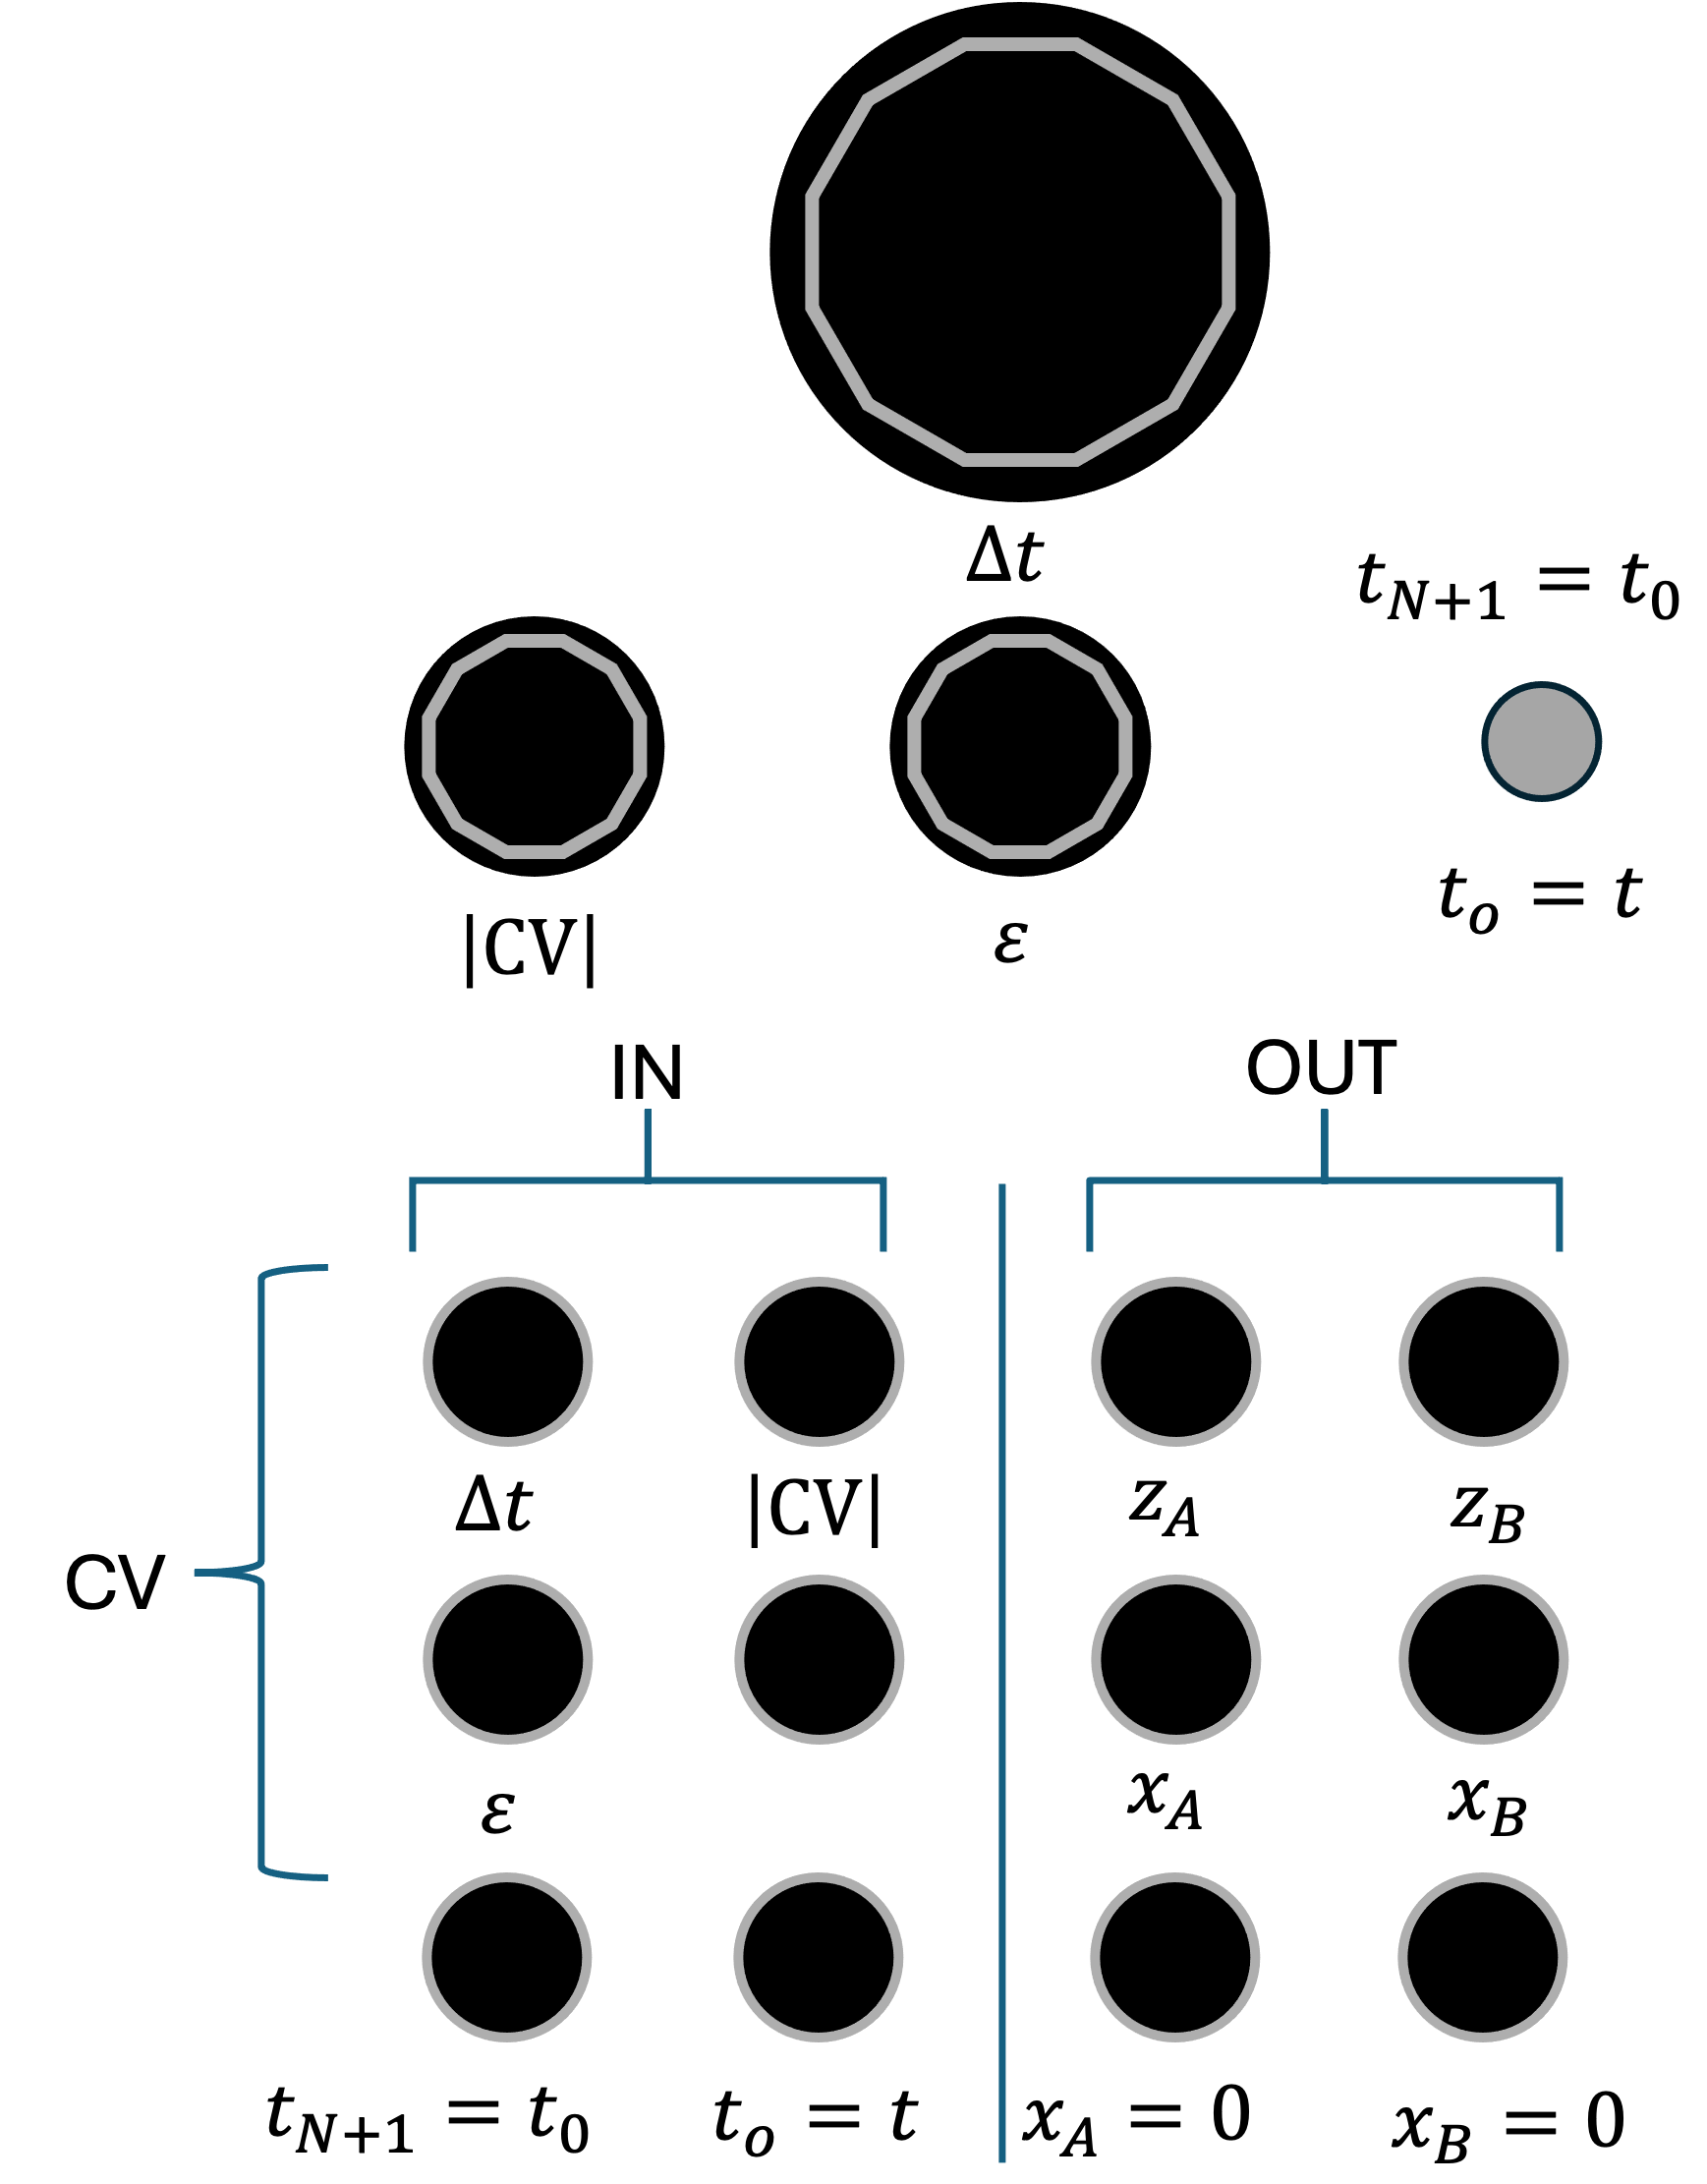
\includegraphics[width=\linewidth]{module_labels.png}%
  \caption{The labels of the Computer's faceplate. The CV inputs control the rate and "randomness" properties shared by the two Lorenz systems, the CV/Audio inputs control the magnitude of the output from each of the two systems, and the switch and pulse inputs allow control of the looping behaviour. The CV outputs provide the $x$- and $z$-coordinates of the trajectories of $A$ and $B$, while the pulse outputs fire when the trajectories of $A$ and $B$ cross zero along the $x$-axis.}%
  \label{fig:module_labels}%
\end{figure}

\subsection{Lorenz System Control Voltages}

The trajectories of the system evolve according to the specified rate for $A$, and are made available as bipolar control voltage signals at the CV and CV/Audio output sockets of the Computer, with the Computer's full range of approximately -6 to +6 V. The rate of $A$ is controlled by the Main knob and the left-most CV input (accepting a range of -5 to +5 V); if a jack is inserted into the left-most CV input the main knob is disconnected and the CV input controls the rate. The two Lorenz systems produce three trajectories each for a total of six, however only four CV output sockets can be used to send the trajectories out of Computer. Given the strong similarity between the trajectories of $x$ and $y$ (see Fig. 2), variables $x$ and $z$ are chosen as the output for each system. This allows plotting of the classic Lorenz butterfly in two dimensions, and the creation of sound pictures of the same. The X-knob acts as an overall attenuator for the four CV outputs, although is disconnected from A or B if a jack is plugged into their respective CV magnitude sockets (the CV/Audio inputs). If a jack is plugged into the left-most CV/Audio input, its (unipolar, 0 to 5 V) value will control the magnitude of the output from system $A$. If a jack is plugged into the right-most CV/Audio input, its (unipolar, 0 to 5 V) value will control the magnitude of the outputs from system $B$. This gives an effective VCA over the CV output, which can be controlled with an envelope (e.g. from the Slopes module of the Workshop System). \marginnote{If using the Slopes module to envelope the CV outputs, note that Slope outputs between 0 and ~9 V, so the upper part of the envelope will not be felt by the magnitude CV input.}

%\begin{figure}[h]
 % 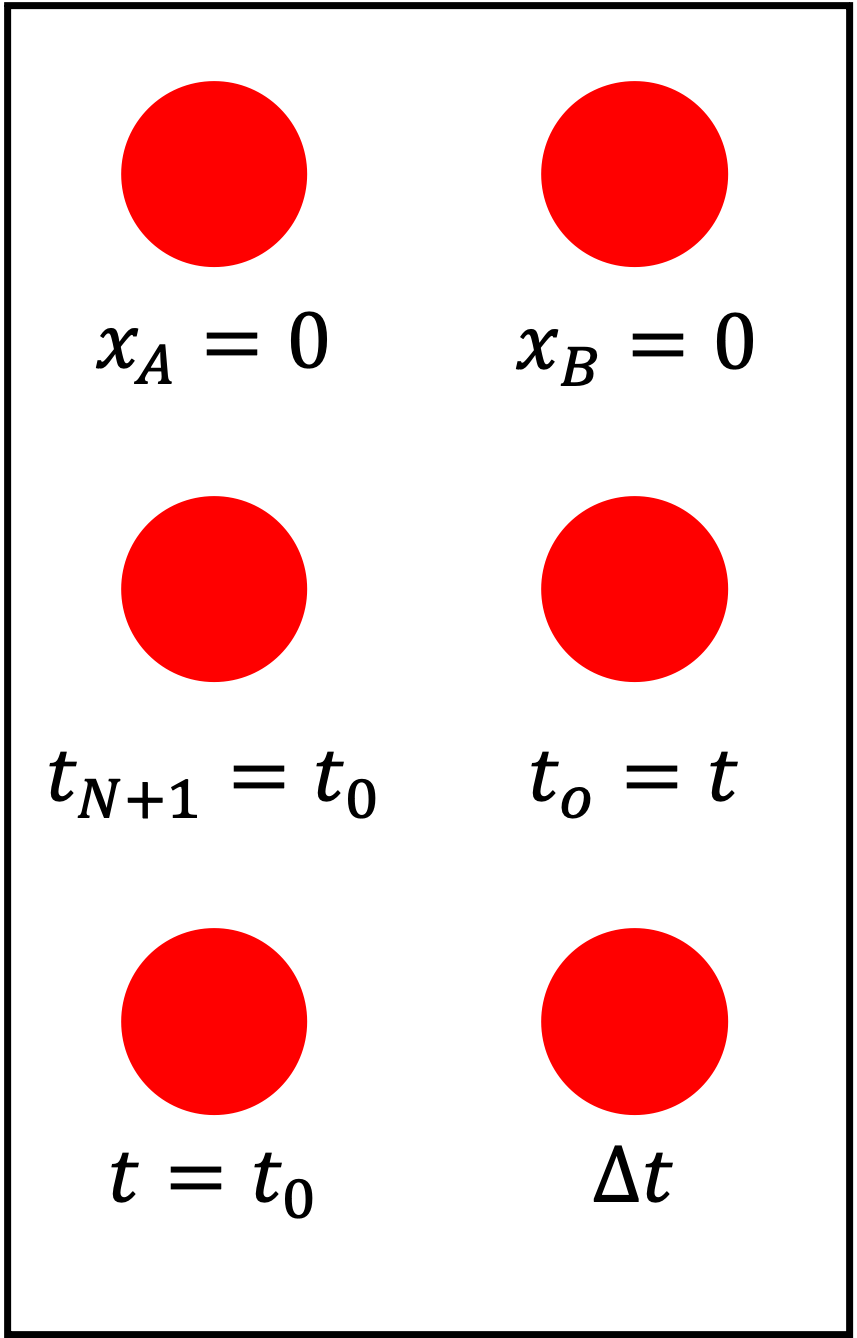
\includegraphics[width=\linewidth]{led_labels.png}%
 % \caption{The functions of the LEDs.}%
 % \label{fig:led_labels}%
%\end{figure}

\subsection{Lorenz System Pulses}

The two pulse outputs of the computer fire whenever the $x$-coordinate of the associated Lorenz system crosses zero. Examining the plot of the trajectories shows that this will produce a rhythm that feels random, although it is completely deterministic. The combination of zero-crossing triggers from the two Lorenz systems will provide contrasting fast and slow rhythms. The top row of LEDs is used to show when the pulses are fired, left is the slower system and right the faster system.

\subsection{Looping}\label{sec:looping}

\newthought{It would be wasteful} to implement a digital module simulating the Lorenz system without making use of the fact that these dynamical systems are highly sensitive to initial conditions. This implies that two trajectories whose starting positions differ by a small amount will initially behave similarly, but over time will drift apart.
This property of similarity of trajectory suggests the idea of returning to the start of a given trajectory, but making a perturbation to the initial position before starting to compute the trajectory again. The magnitude of this perturbation will determine for how long the first and second solutions of the system will remain similar before diverging.

\begin{figure*}[h]
  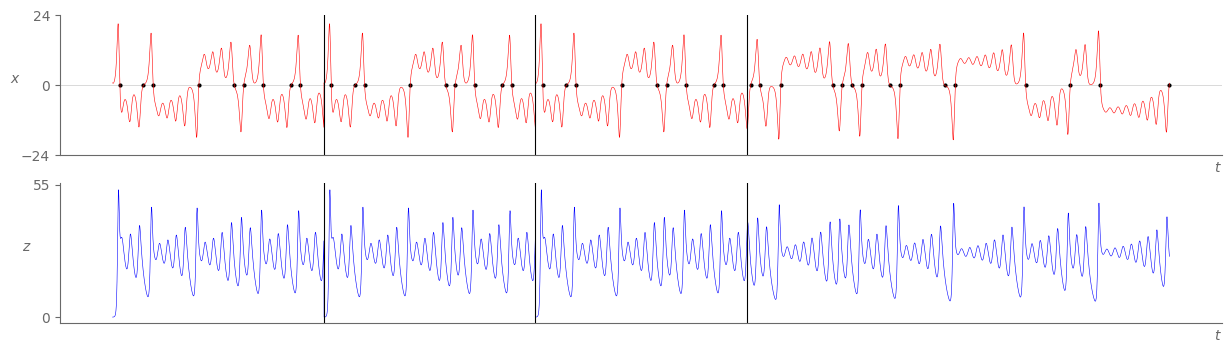
\includegraphics[width=\linewidth]{looping_voltages.png}%
  \caption{Looping the two Lorenz systems (without sensitivity to initial conditions). The simulation starts at an arbitrary $t_0$ and begins looping at $t_n$, marked with a black line. After the second repeat, looping ends and the trajectory evolves freely.}%
  \label{fig:looping_voltages}%
\end{figure*}

This idea is also based on the concept that repeating randomness becomes not random at all. While the trajectories are not "random" in any sense - they are in fact completely deterministic - they are not repetitive in an obvious way and give a sense of back-and-forth evolution. It is not predictable to a listener when or how quickly the system will move from one attractor to another, or how long an orbit on an attractor will last. However, if a section of the trajectory is repeated over a short enough time range, the repetition will become obvious to the listener. Thus, we can take an unpredictable system and make it predictable by looping a section of a trajectory between an initial position $x_0, y_0, z_0$ and a final position $x_N, y_N, z_N$ where $N$ is the number of steps taken between the initial and final positions (see Fig. 4). 

\begin{figure*}[h]
  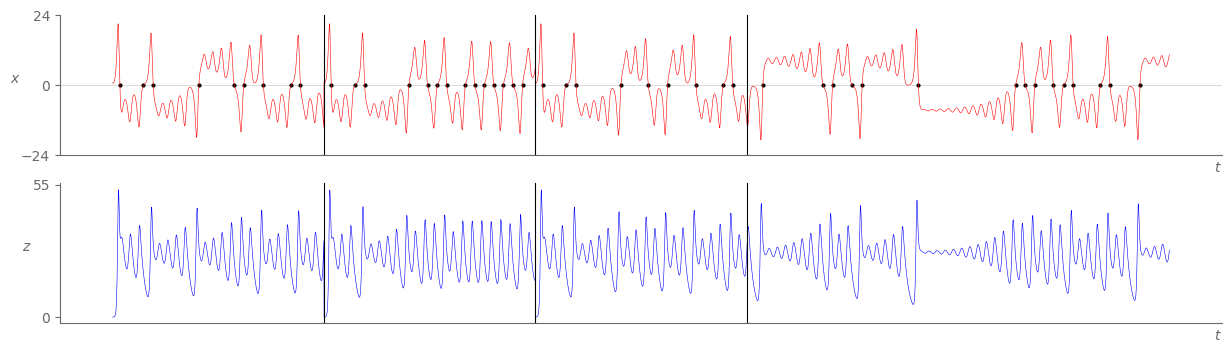
\includegraphics[width=\linewidth]{dependent_loop.png}%
  \caption{Looping the two Lorenz systems with sensitivity to initial conditions. At each repeat (marked with a black line) the trajectory initially appears similar, by approximately halfway through the loop the trajectory becomes different. After three repeats the loop is released.}%
  \label{fig:dependent_loop}%
\end{figure*}

Given this loop, the sensitivity to initial conditions can be made useful. By allowing the musician to control the magnitude of a random perturbation added to the initial position, the loop can be tuned to be either the same every time ($\zeta=0$), or to diverge on each repeat to a desired degree ($\zeta$ between 0 and 2, chosen by considered listening). This opens the door to a fuzzier definition of repetition where the loop is "similar enough" each time for the listener to detect repetition, but different enough to remain somewhat unpredictable, at the direction of the musician (see Fig. 5). This effect will also be felt on the pulse outputs. 

\begin{figure*}[h]
  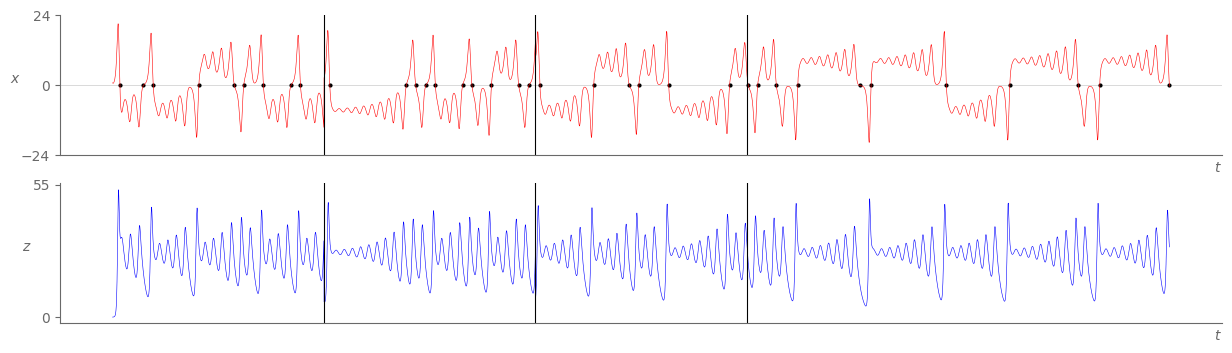
\includegraphics[width=\linewidth]{very_dependent_loop.png}%
  \caption{Looping the two Lorenz systems with a high degree of sensitivity to initial conditions. In this case, each loop has little similarity to any other, and the system is effectively evolving as if looping is diengaged.}%
  \label{fig:very_dependent_loop}%
\end{figure*}

The Y-knob is used to set the amount of randomness. If a jack is plugged into the right-most CV input (-5 to +5 V), the value at the jack will control the value of the randomness, and the Y-knob will be disconnected.

Looping can also be controlled via the pulse inputs. The start point is set by sending a trigger into the leftmost pulse input or clicking the Z-switch down. This will store the postition at which the trigger (or switch click) was detected as $r_0$, and begin counting steps on the trajectory. Looping can be controlled either by a trigger at the rightmost pulse input or by setting the Z-switch to the up position (middle corresponds to turning looping off). The goal of including the switch is playability of the loop, and the trigger enables some amount of repeatability. When looping is turned on, the position at the current time is used as $r_N$ and the system will immediately return to $r_0$, evolving until the number of steps $N$ has elapsed then returning to $r_0$. Turning looping off un-loops the time circle back to a flat line and the system will continue to freely evolve without affecting $t_0$; $t_N$ is forgotten at the point looping is turned off (see Figs. 4, 5 and 6).

The centre row of LEDs shows the loop status. The leftmost LED is lit when looping is enabled, and the rightmost flashes when the loop start point $r_0$ is set. The bottom row of LEDs flash when the loop boundary is crossed (i.e. at the simultaneous start/end of the loop $t_0$).


\section{Future Work}\label{sec:future_work}

The implementation of Od takes care to avoid stable solutions of the Lorenz system (i.e. those with $\rho < 1$, or $\rho > 1$ where the stability test is able to confirm stability of the system. This in done to ensure the outputs of the module are chaotic. However, stable solutions could provide interesting, loop-able decaying oscillatory envelopes. This could be incorporated in Od or act as the basis for a separate module or half-program of Computer.

The assumption that the Euler method is sufficient for solving the Lorenz system warrants further investigation, and the implementation of a method with smaller error could be attempted. This could permit a longer maximum timestep allowing access to faster rates, but any improvement will be balanced with the higher expense of evaluating the system trajectory.


\bibliography{sample-handout}
\bibliographystyle{plainnat}



\end{document}
